% !TEX encoding = UTF-8 Unicode
% !TEX root = thesis-ex.tex

A pileup event is an event in which there are multiple \pbpb\ interactions.
The rate of such events is typically minimized in a heavy ion collision by increasing the crossing angle between the colliding beams.
Pileup events are further rejected by identifying them using information from the tracking systems and by studying the correlation between the energy deposited in the ZDC and the FCal.
In heavy ion collisions, all tracks in the tracking system are fit back to a single primary vertex with the fits that do not converge being rejected.
Then events that have a track multiplicity corresponding to a single \pbpb\ interaction and an energy deposition in the calorimeter that is consistent with multiple \pbpb\ interactions are pileup events~\cite{Aad2014}.
Pileup events are also identified using the anti-correlation between the number of participant and spectator nucleons in a heavy ion collision.
Figure~\ref{fig:zdc_fcal} shows the total energy in the ZDC normalized by the energy of a single neutron vs. the sum of transverse energy in the FCal, \ETfcal.
The former comes from spectators of the collision, while the latter from the participants.
Events in which the ZDC measures more neutrons than expected for a given energy in the FCal are then identified as pileup events.

\begin{figure}[ht]
	\centering
        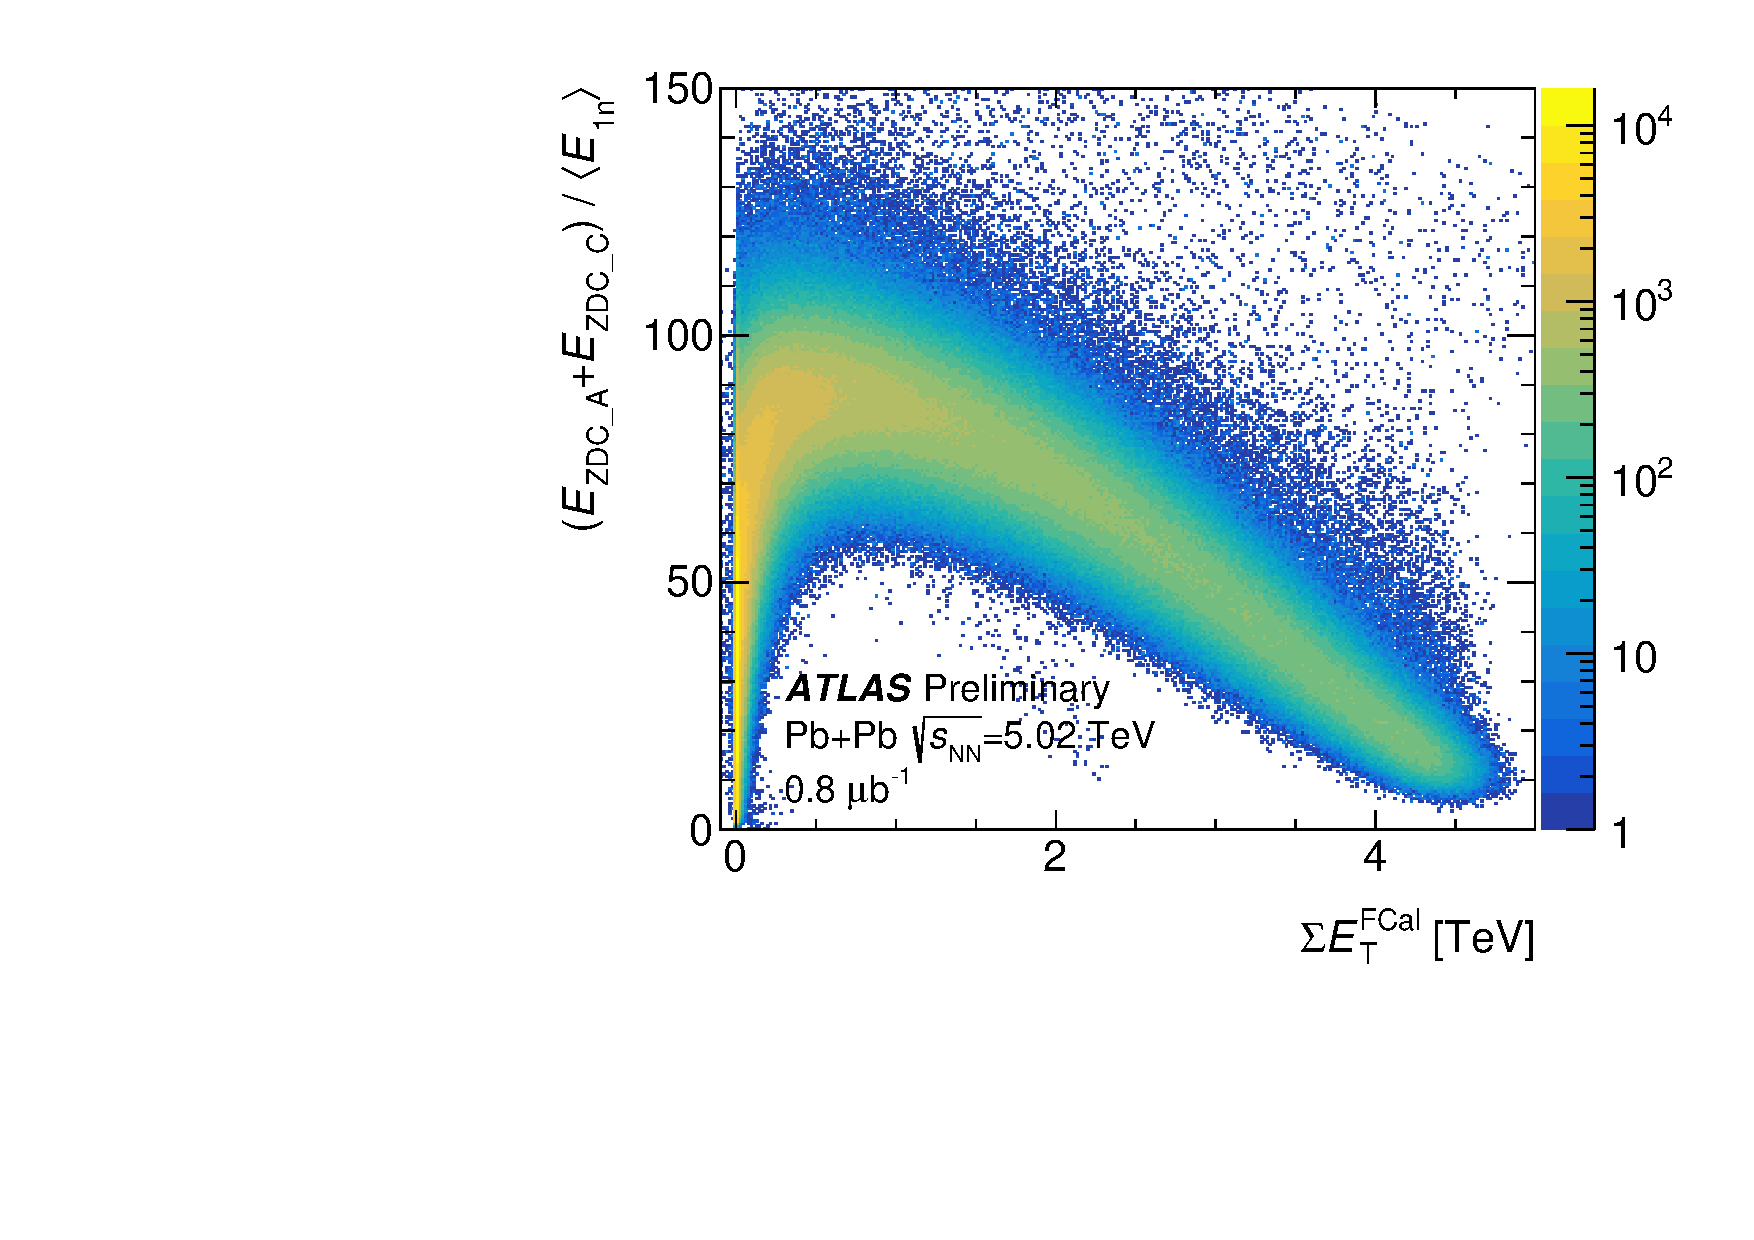
\includegraphics[width=0.5\textwidth]{figures/setup/zdc_fcal}
          \caption{The correlation of the sum of energies in the ZDC arms vs. the sum of transverse energies in the FCal.
          Multiple \pbpb\ interactions in the same beam crossing with at least one of them being a central collision would deposit large amounts of energy in the FCal and the ZCD, and are seen as the grass near the top right of the figure.
          This is used to identify pileup events.
           Figure taken from Ref.~\cite{perfPlots}.}
          \label{fig:zdc_fcal}
\end{figure}


Once pileup events have been identified and removed, the event centrality can be determined.
This is done by coupling information from the Glauber Model with signals from the ZDC and FCal \cite{ATLAS:2016tor, Aaboud:2018ves}.
The centrality of an event can be mapped to the charged particle multiplicity $N_{\rm ch}$ using the Glauber Model as was shown in Figure~\ref{fig:cent_estimate}.
It can also be seen from Figure~\ref{fig:nch_fcal} that the charged particle multiplicity is strongly correlated with \ETfcal.
Then an MC Glauber simulation can be used to describe the \ETfcal\ distribution shown in Figure~\ref{fig:fcal_distr}, and divide it into percentiles \cite{ATLAS:2011ah}.
The 0--10\% centrality corresponds to most central collisions with the maximum overlap between the colliding nuclei, while the 90--100\% corresponds to the most peripheral collisions with the least overlap between the colliding nuclei.
Since the energy in the barrel region ($|\eta| < 3.2$) is highly correlated with the energy in the FCal ( $3.2 < |\eta| < 4.9$) as shown in Figure~\ref{fig:fcal_barrel}, using different regions of the detector to estimate event centrality and conduct measurements ensures a consistent centrality determination while avoiding autocorrelations in the analysis.



\begin{figure}
\centering
\begin{subfigure}{.45\textwidth}
  \centering
  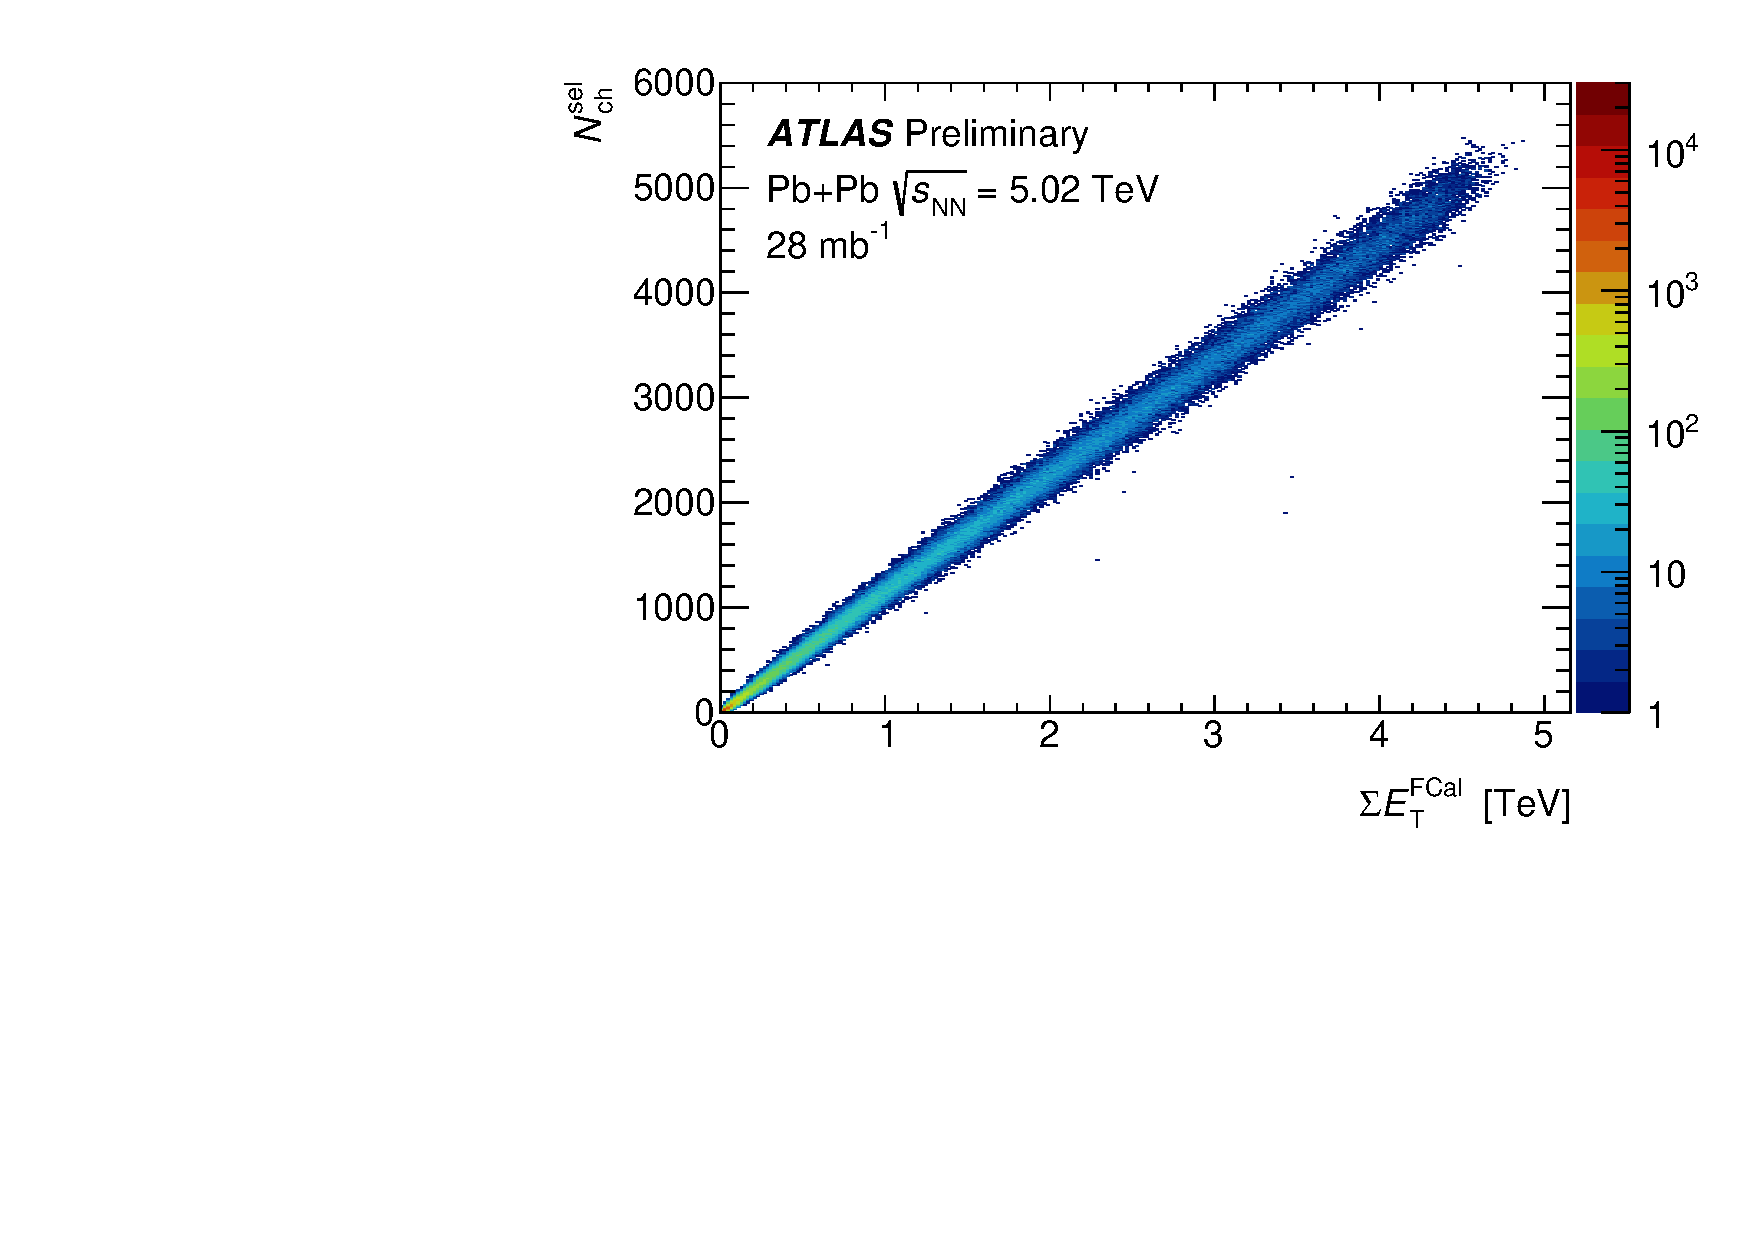
\includegraphics[width=\linewidth]{figures/setup/nch_fcal}
          \caption{}
          \label{fig:nch_fcal}
\end{subfigure}
\qquad  \qquad  
\begin{subfigure}{.45\textwidth}  
  \centering
  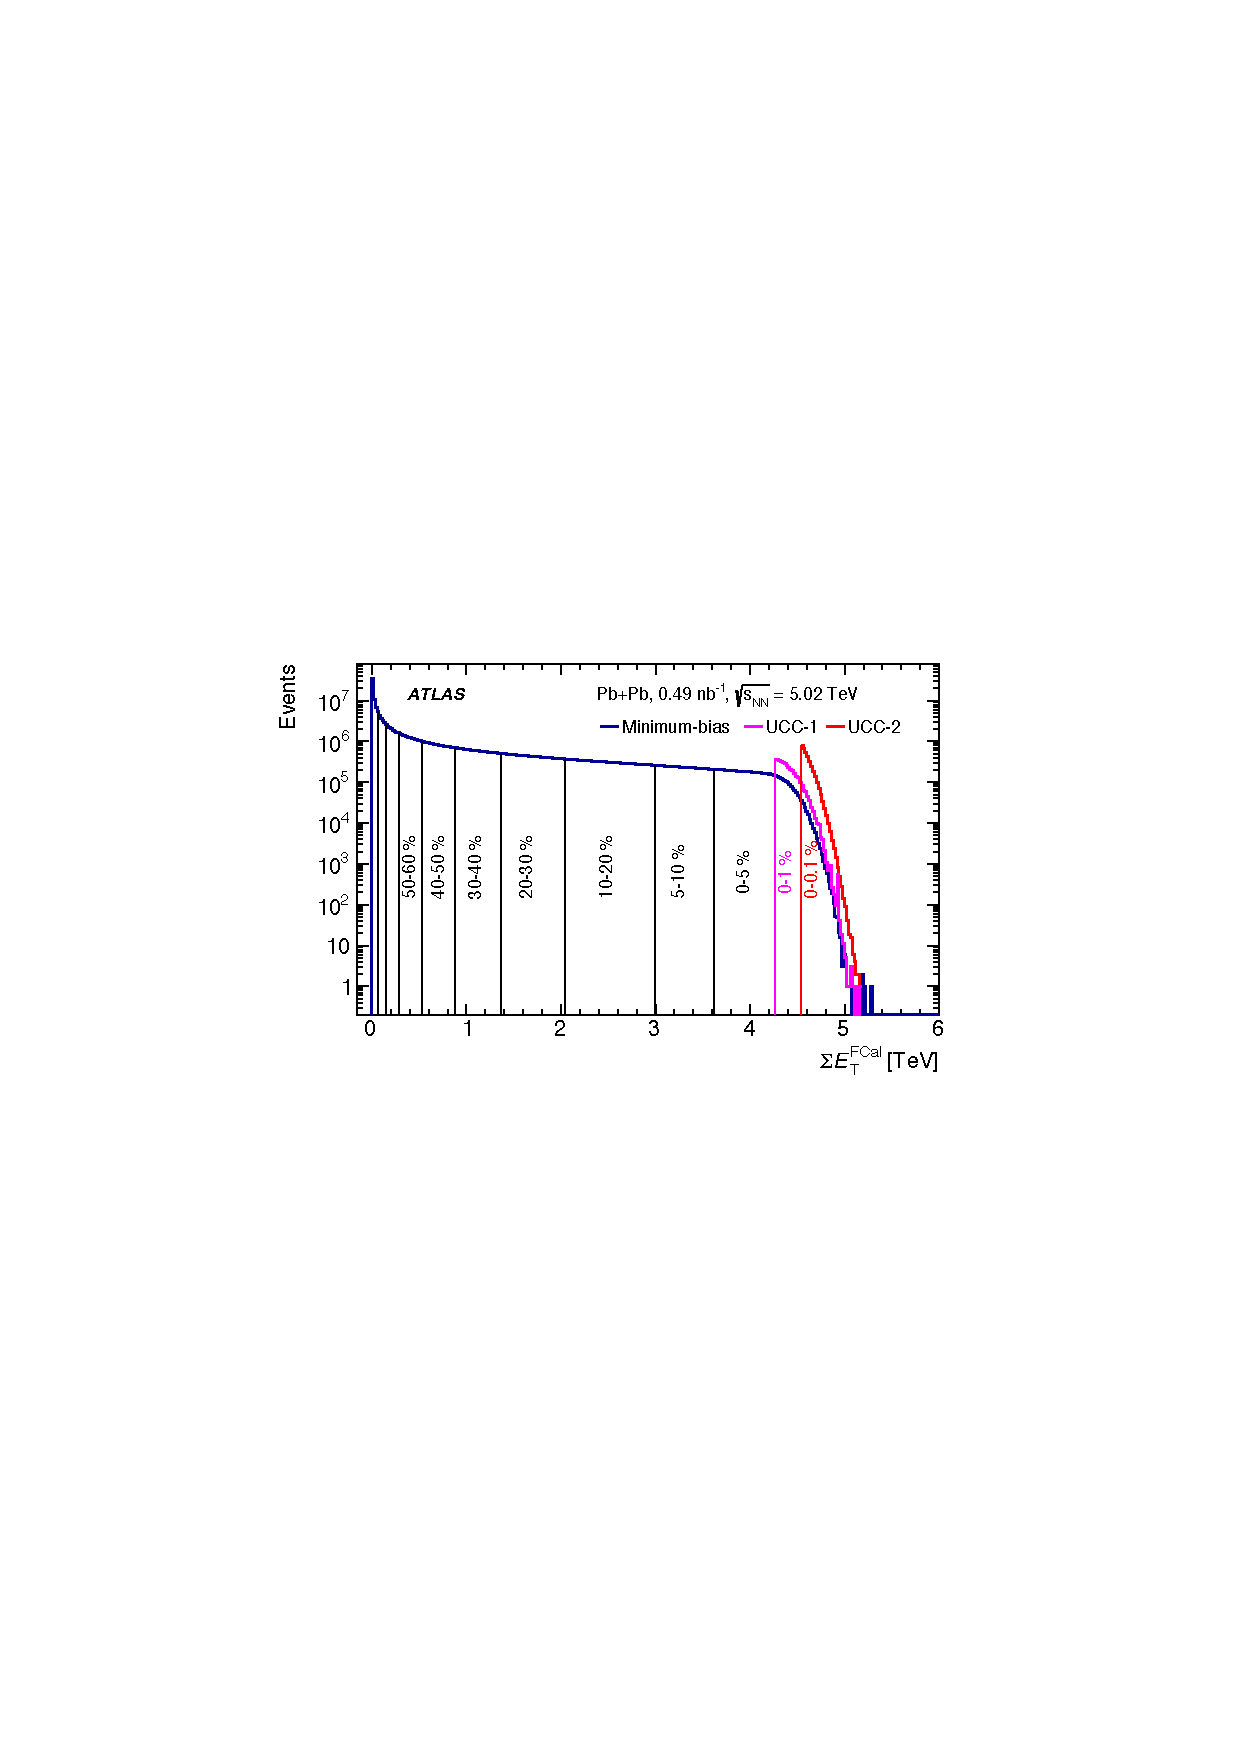
\includegraphics[width=\linewidth]{figures/setup/fcal_distr}
          \caption{}
          \label{fig:fcal_distr}
\end{subfigure}
\caption{(Left) Charged particle multiplicity $N_{\rm ch}^{\rm sel}$ versus the total transverse energy in the FCal, \ETfcal.
Taken from Ref.~\cite{perfPlots}.
(Right) The \ETfcal\ distribution for events selected by the minimum bias trigger along with the centrality percentiles.
Also shown are the number of events over the 0--1\% and 0--0.1\% centrality intervals selected by the ultra-central triggers.
Figure taken from Ref.~\cite{Aaboud:2018ves}.
Both plots are for \pbpb\ collisions with $\sqrtsnn = 5.02$ TeV.}
\label{}
\end{figure}


\begin{figure}[ht]
	\centering
        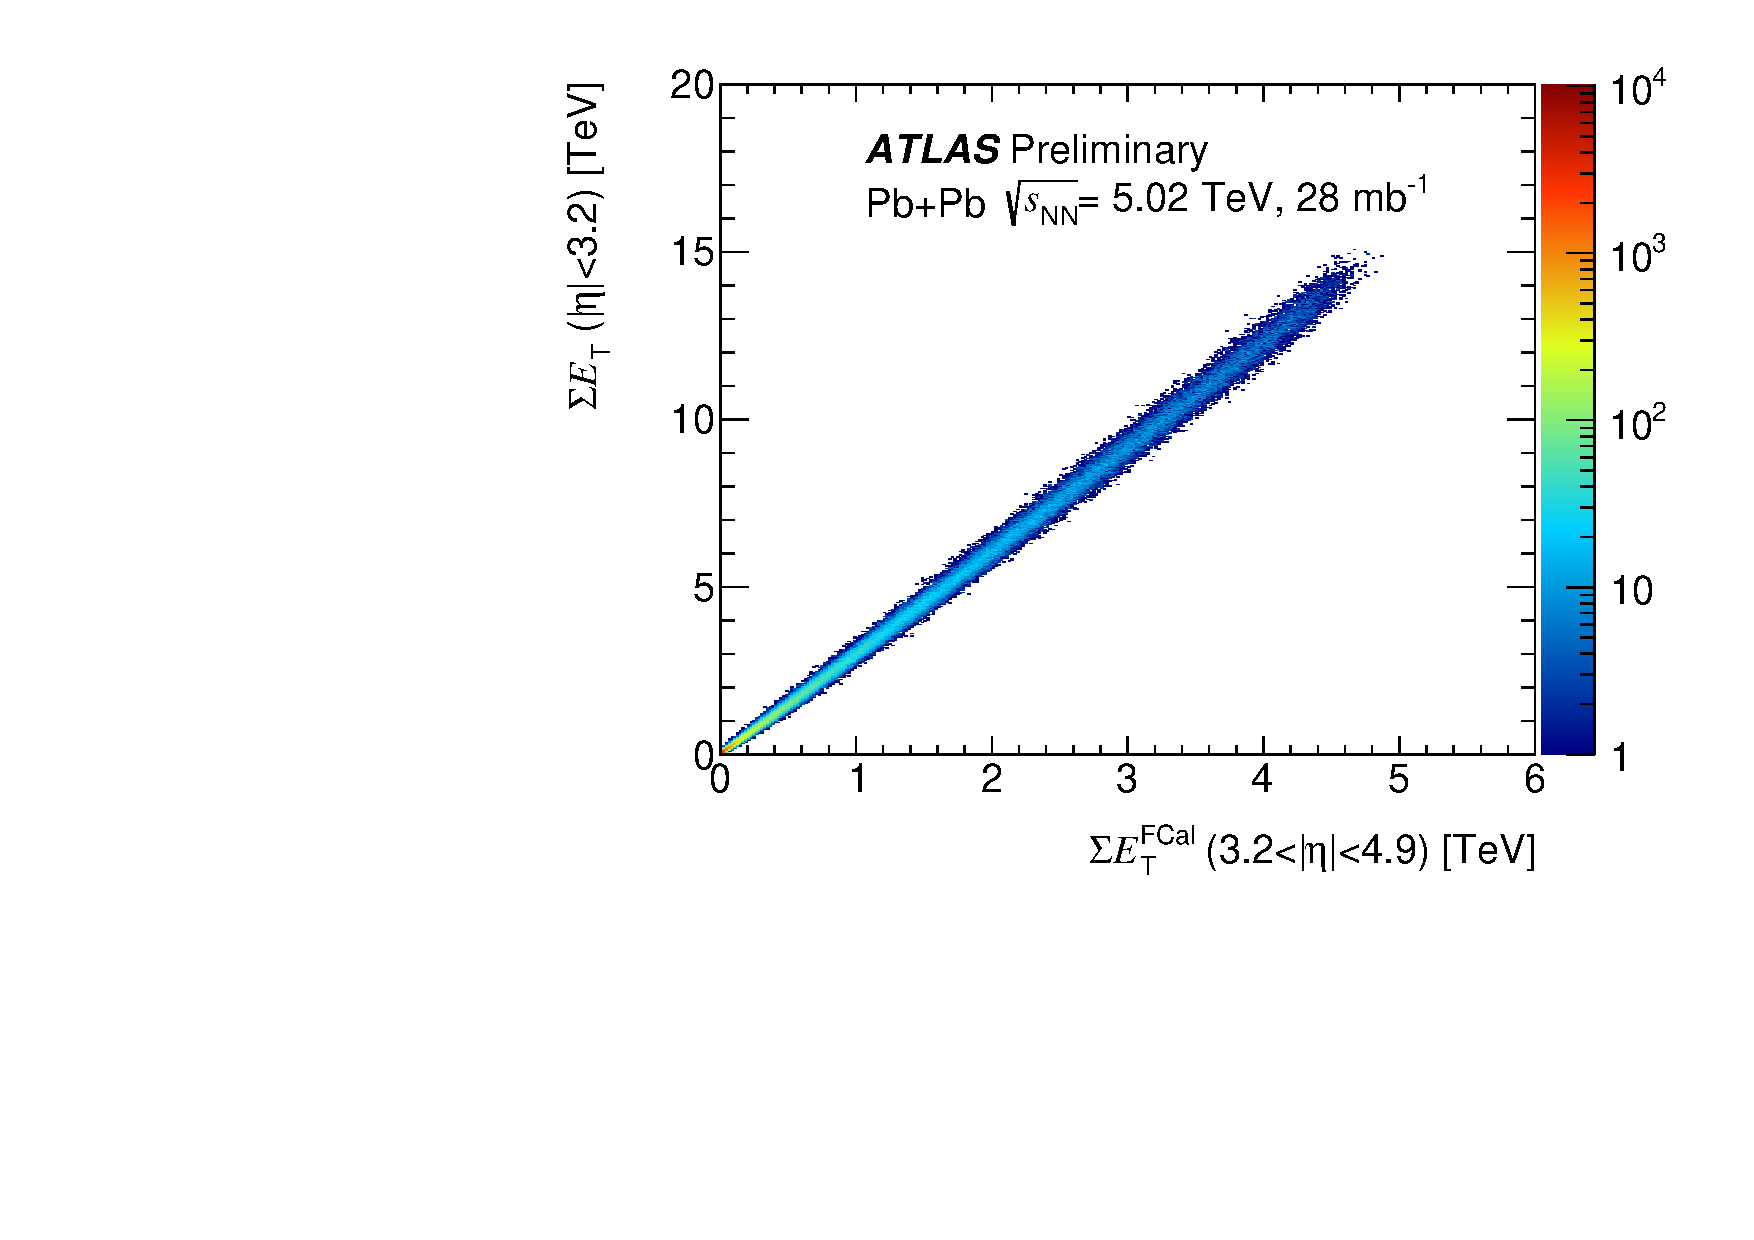
\includegraphics[width=0.5\textwidth]{figures/setup/fcal_barrel}
          \caption{Correlation of the total energy in the calorimeter in the interval of $|\eta| < 3.2$ with the total energy measured in the forward calorimeters for \pbpb\ collisions with $\sqrtsnn = 5.02$ TeV.
          Taken from Ref.~\cite{perfPlots}.}
          \label{fig:fcal_barrel}
\end{figure}


